\section{Results}\label{sec:results}

\subsection{Effect of the Evaluation Design}

The accuracy of every model on complete data is given for the three designs in
Table~\ref{tab:e1} and Fig.~\ref{fig:e1}. Under the random split used in most earlier studies,
the random forest was the most accurate model for every crop ($R^2$ of 0.41 for groundnut, 0.31
for bajra and 0.38 for wheat), followed by XGBoost or ridge regression, and all models clearly
outperformed the mean predictor. Averaged over the crops, $R^2$ fell from 0.37 to 0.29 for the
random forest, from 0.32 to 0.24 for XGBoost and from 0.31 to 0.19 for ridge regression when
whole districts were held out, which corresponds to an increase of 2.0 to 2.6 pp in nRMSE. The
bootstrap over districts confirmed that this loss is not caused by chance for groundnut and bajra:
for the random forest, the RMSE rose by 0.044~t/ha (95\% CI [0.012, 0.087]) for groundnut and by
0.063~t/ha ([0.034, 0.088]) for bajra, that is, by 7 and 14\% of the random-split error. For
wheat, the loss was significant for ridge regression but not for the tree ensembles, whose
intervals included zero.

The temporal split was the most difficult design. The tree ensembles reached a negative $R^2$ on
the seasons 2016--17 to 2022--23 for groundnut and bajra and fell to 0.19 (random forest) and
0.06 (XGBoost) for wheat. Ridge regression was the best model under this design (crop mean
$R^2 = 0.04$ against $-0.04$ for the ensembles), because yields rose over time and a linear year
term extrapolates this trend, whereas the predictions of a tree ensemble cannot leave the range
of the training yields. Even the best model explained little variation among the later seasons,
whose mean was itself higher than the training mean, so the mean predictor obtained a strongly
negative $R^2$ ($-0.68$).

\begin{table}[!t]
\caption{Accuracy on Complete Data Under the Three Evaluation Designs (RMSE in t/ha, Mean of
Three Seeds)}\label{tab:e1}
\centering\footnotesize\setlength{\tabcolsep}{4pt}
\begin{tabular}{lrrrrrr}
\toprule
 & \multicolumn{2}{c}{Random split} & \multicolumn{2}{c}{Temporal} & \multicolumn{2}{c}{District holdout} \\ \cmidrule(lr){2-3}\cmidrule(lr){4-5}\cmidrule(lr){6-7}Model & RMSE & $R^2$ & RMSE & $R^2$ & RMSE & $R^2$ \\
\midrule
\multicolumn{7}{l}{\textit{Groundnut}} \\
Mean & 0.837 & $-$0.01 & 1.082 & $-$1.05 & 0.839 & $-$0.01 \\
Ridge & 0.676 & 0.34 & 0.757 & $-$0.00 & 0.695 & 0.31 \\
RF & 0.640 & 0.41 & 0.802 & $-$0.12 & 0.674 & 0.35 \\
XGB & 0.666 & 0.36 & 0.766 & $-$0.03 & 0.697 & 0.30 \\
\multicolumn{7}{l}{\textit{Bajra}} \\
Mean & 0.573 & $-$0.01 & 0.739 & $-$0.57 & 0.592 & $-$0.07 \\
Ridge & 0.501 & 0.23 & 0.569 & 0.07 & 0.551 & 0.07 \\
RF & 0.472 & 0.32 & 0.638 & $-$0.17 & 0.509 & 0.20 \\
XGB & 0.494 & 0.25 & 0.632 & $-$0.15 & 0.541 & 0.10 \\
\multicolumn{7}{l}{\textit{Wheat}} \\
Mean & 0.688 & $-$0.00 & 0.769 & $-$0.43 & 0.699 & $-$0.04 \\
Ridge & 0.549 & 0.36 & 0.628 & 0.05 & 0.621 & 0.18 \\
RF & 0.540 & 0.38 & 0.578 & 0.19 & 0.572 & 0.31 \\
XGB & 0.559 & 0.34 & 0.624 & 0.06 & 0.571 & 0.31 \\
\bottomrule
\end{tabular}

\end{table}

\begin{figure*}[!t]
\centering
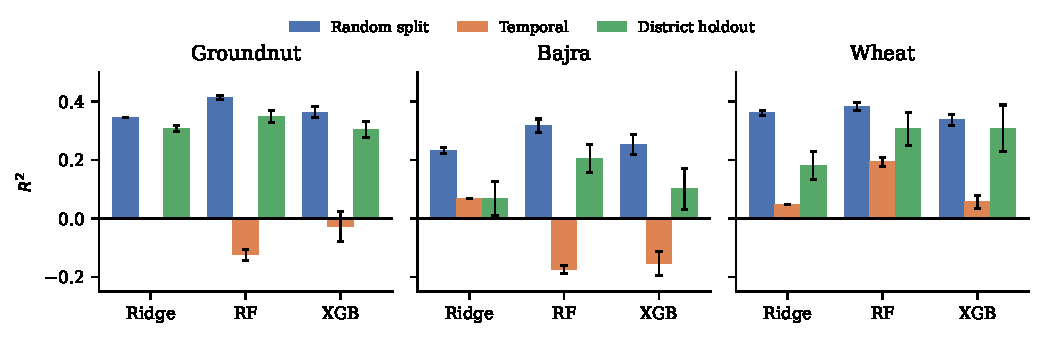
\includegraphics[width=0.82\textwidth]{fig_e1_designs}
\caption{$R^2$ on complete data under the three evaluation designs (error bars: standard deviation
over three seeds). The mean predictor is omitted for readability; its values are given in
Table~\ref{tab:e1}.}
\label{fig:e1}
\end{figure*}

\subsection{Effect of Missing Weather Data}

The rise in nRMSE caused by missing weather in unseen districts is plotted against the missingness
rate in Fig.~\ref{fig:e2}, and the values at 30\% are given for all ten strategies in
Table~\ref{tab:e2}. The damage generally grew with the rate but remained moderate: at 40\%, the
nRMSE of the ensembles rose by 0.9 to 1.6 pp, which is less than the 2.0 to 2.1~pp lost by moving from
familiar to unseen districts. Variable-wise missingness was the most harmful pattern at 30\%
(1.1 to 1.5 pp for the ensembles), because a whole group of related features, such as all rainfall
features, is removed at once and cannot be estimated from its neighbours. Under random masking,
iterative and KNN imputation preserved accuracy better than median replacement for every model:
for the random forest, the damage at 30\% was 0.4~pp with iterative imputation and 0.8~pp with the
median. Block outages behaved differently. At 30\%, only 10.6\% of the feature values became
missing, but most features were estimated from fewer days; the damage was then similar for all
imputers (0.6 to 0.9~pp for the ensembles), since the main error lies in the distorted values that
no imputer replaces. At 10\%, where no values became missing, the error of the ensembles even
decreased slightly (by 0.3~pp), which is within the variation between seeds.

\begin{figure*}[!t]
\centering
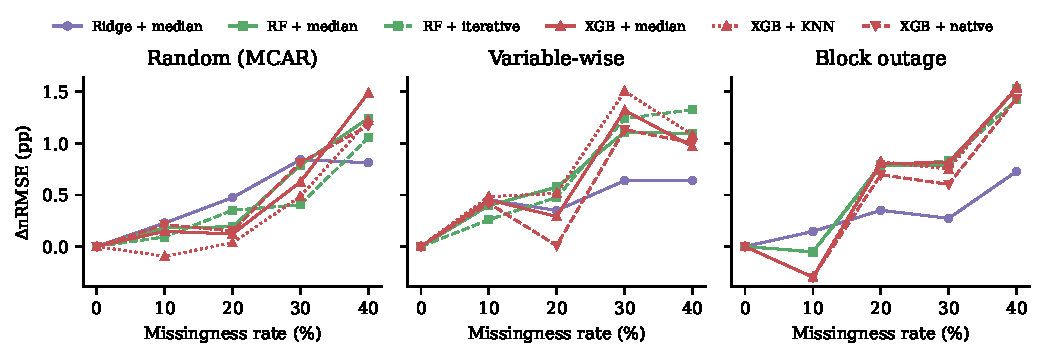
\includegraphics[width=0.82\textwidth]{fig_e2_degradation}
\caption{Rise in nRMSE relative to complete data under the district holdout, averaged over the
three crops and three seeds, for selected model--strategy combinations.}
\label{fig:e2}
\end{figure*}

\begin{table}[!t]
\caption{Damage at 30\% Missingness Under the District Holdout ($\Delta$nRMSE in pp and $R^2$,
Mean Over Crops)}\label{tab:e2}
\centering\footnotesize\setlength{\tabcolsep}{3.5pt}
\begin{tabular}{lrrrrrr}
\toprule
 & \multicolumn{2}{c}{Random (MCAR)} & \multicolumn{2}{c}{Variable-wise} & \multicolumn{2}{c}{Block outage} \\ \cmidrule(lr){2-3}\cmidrule(lr){4-5}\cmidrule(lr){6-7}Strategy & $\Delta$nRMSE & $R^2$ & $\Delta$nRMSE & $R^2$ & $\Delta$nRMSE & $R^2$ \\
\midrule
Ridge + median & 0.8 & 0.13 & 0.6 & 0.14 & 0.3 & 0.17 \\
Ridge + KNN & 0.5 & 0.15 & 0.7 & 0.14 & 0.1 & 0.17 \\
Ridge + iterative & 0.3 & 0.17 & 0.4 & 0.15 & 0.3 & 0.17 \\
RF + median & 0.8 & 0.25 & 1.1 & 0.23 & 0.8 & 0.25 \\
RF + KNN & 0.5 & 0.26 & 1.4 & 0.22 & 0.8 & 0.25 \\
RF + iterative & 0.4 & 0.26 & 1.2 & 0.22 & 0.8 & 0.25 \\
XGB + median & 0.6 & 0.20 & 1.3 & 0.17 & 0.8 & 0.20 \\
XGB + KNN & 0.5 & 0.21 & 1.5 & 0.16 & 0.7 & 0.20 \\
XGB + iterative & 0.4 & 0.21 & 1.4 & 0.16 & 0.9 & 0.19 \\
XGB + native & 0.8 & 0.19 & 1.1 & 0.18 & 0.6 & 0.21 \\
\bottomrule
\end{tabular}

\end{table}

Ridge regression was damaged least by every pattern (0.1 to 0.8~pp), but it started from a much
lower accuracy, and its $R^2$ under missingness (0.13 to 0.17) remained below that of every
ensemble under the same pattern. When the ten strategies were ranked within each of the 36 combinations of crop, pattern
and rate, the three random-forest strategies took the first three places (average ranks 1.96 for
iterative, 2.10 for KNN and 2.14 for median imputation), the XGBoost strategies followed (6.46 to
6.96) and the ridge strategies came last (7.14 to 7.81); the differences were highly significant
(Friedman $\chi^2 = 205.1$, $p < 10^{-38}$). The choice of model therefore mattered much more than
the choice of imputer. Against native missing-value handling in XGBoost, the random forest with
iterative imputation was significantly more accurate in six of the nine combinations of crop and
pattern at 30\% (bootstrap over districts), but against the random forest with median replacement
it differed significantly in only two, once in each direction.

\subsection{Combined Effect of Missing Data and Geographic Shift}

The geographic, missingness and combined effects of \eqref{eq:inter} are given at 30\%
missingness in Table~\ref{tab:inter}. Contrary to the third hypothesis, the combined loss was
\emph{smaller} than the sum of the separate losses for almost every strategy and pattern: the
interaction averaged $-0.4$~pp and was significantly below zero ($t = -3.85$, $p < 0.001$, 45
combinations). For example, for the random forest with median replacement and random masking, the
geographic shift cost 2.1~pp and missingness 1.3~pp, but both together only 2.9~pp. The
interaction was negative for groundnut ($-0.6$~pp) and bajra ($-0.9$~pp) and slightly positive for
wheat ($+0.3$~pp). One explanation is that both problems remove the same information: a model
applied to an unseen district cannot rely on the fine weather patterns specific to that district,
so losing part of these patterns to missingness costs less than it does in familiar districts.

\begin{table}[!t]
\caption{Geographic (Geo.), Missingness (Miss.) and Combined (Comb.) Effects at 30\% Missingness
and Their Interaction (Inter.), in pp of nRMSE, Mean Over Crops}\label{tab:inter}
\centering\footnotesize\setlength{\tabcolsep}{3.5pt}
\begin{tabular}{llrrrr}
\toprule
Strategy & Pattern & Geo. & Miss. & Comb. & Inter. \\
\midrule
Ridge + median & Random (MCAR) & 2.6 & 1.4 & 3.4 & $-$0.6 \\
Ridge + median & Variable-wise & 2.6 & 1.0 & 3.2 & $-$0.4 \\
Ridge + median & Block outage & 2.6 & 1.0 & 2.8 & $-$0.7 \\
RF + median & Random (MCAR) & 2.1 & 1.3 & 2.9 & $-$0.5 \\
RF + median & Variable-wise & 2.1 & 1.5 & 3.2 & $-$0.4 \\
RF + median & Block outage & 2.1 & 1.2 & 2.8 & $-$0.4 \\
RF + iterative & Random (MCAR) & 2.1 & 0.5 & 2.5 & $-$0.1 \\
RF + iterative & Variable-wise & 2.1 & 1.4 & 3.3 & $-$0.1 \\
RF + iterative & Block outage & 2.1 & 1.2 & 2.9 & $-$0.3 \\
XGB + median & Random (MCAR) & 2.0 & 1.4 & 2.6 & $-$0.7 \\
XGB + median & Variable-wise & 2.0 & 1.3 & 3.3 & 0.0 \\
XGB + median & Block outage & 2.0 & 1.0 & 2.8 & $-$0.2 \\
XGB + native & Random (MCAR) & 2.0 & 1.3 & 2.8 & $-$0.5 \\
XGB + native & Variable-wise & 2.0 & 1.5 & 3.1 & $-$0.4 \\
XGB + native & Block outage & 2.0 & 1.1 & 2.6 & $-$0.5 \\
\bottomrule
\end{tabular}

\end{table}

\subsection{Effect of Feature Selection}

The results of the feature-selection experiment are given in Table~\ref{tab:e3}. With eight
features, the random forest retained almost the same accuracy as with all 18 (nRMSE of 33.9\% with
mutual information and 34.1\% with recursive elimination, against 33.9\%), but it was not made more
robust: at 40\% missingness, the full set remained at least as accurate (35.1\% against 35.1 and
35.3\%). XGBoost lost 0.4 to 1.0~pp with either reduced set. The year was selected in all 15 folds
by both methods, followed by wind speed, humidity and mid-season rainfall; hot days were often
chosen by mutual information (10 folds) but rarely by recursive elimination (1 fold).

\begin{table}[!t]
\caption{Feature Selection Under the District Holdout and MCAR Missingness (nRMSE in \% and $R^2$,
Mean Over Crops)}\label{tab:e3}
\centering\footnotesize\setlength{\tabcolsep}{2.6pt}
\begin{tabular}{llrrrrrr}
\toprule
 & & \multicolumn{2}{c}{0\%} & \multicolumn{2}{c}{20\%} & \multicolumn{2}{c}{40\%} \\ \cmidrule(lr){3-4}\cmidrule(lr){5-6}\cmidrule(lr){7-8}Strategy & Features & nRMSE & $R^2$ & nRMSE & $R^2$ & nRMSE & $R^2$ \\
\midrule
RF + median & Full (18) & 33.9 & 0.29 & 34.1 & 0.27 & 35.1 & 0.23 \\
RF + median & Mutual info. (8) & 33.9 & 0.28 & 34.4 & 0.26 & 35.1 & 0.22 \\
RF + median & RFE (8) & 34.1 & 0.28 & 34.6 & 0.25 & 35.3 & 0.21 \\
XGB + native & Full (18) & 35.1 & 0.24 & 35.3 & 0.22 & 36.3 & 0.17 \\
XGB + native & Mutual info. (8) & 35.6 & 0.21 & 36.1 & 0.18 & 36.7 & 0.15 \\
XGB + native & RFE (8) & 35.6 & 0.22 & 36.3 & 0.18 & 36.8 & 0.14 \\
\bottomrule
\end{tabular}

\end{table}

\subsection{Effect of Location Features}

Adding the latitude and longitude of the district headquarters changed the tree ensembles little
(crop-mean $R^2$ of 0.29 to 0.28 for the random forest and 0.24 to 0.23 for XGBoost), but improved
ridge regression for every crop (Table~\ref{tab:e4}), from 0.19 to 0.32 on average, so that it
became the most accurate model under the district holdout. A linear model can use a smooth
north--south and east--west gradient to place an unseen district between known ones, whereas the
tree ensembles appear to obtain similar information from the weather features, which already vary
with location.

\begin{table}[!t]
\caption{$R^2$ Without $\rightarrow$ With Location Features, District Holdout}\label{tab:e4}
\centering\footnotesize
\begin{tabular}{lccc}
\toprule
Model & Groundnut & Bajra & Wheat \\
\midrule
Ridge & 0.31 $\rightarrow$ 0.35 & 0.07 $\rightarrow$ 0.28 & 0.18 $\rightarrow$ 0.33 \\
RF & 0.35 $\rightarrow$ 0.37 & 0.20 $\rightarrow$ 0.19 & 0.31 $\rightarrow$ 0.29 \\
XGB & 0.30 $\rightarrow$ 0.35 & 0.10 $\rightarrow$ 0.04 & 0.31 $\rightarrow$ 0.29 \\
\bottomrule
\end{tabular}

\end{table}
